\documentclass[10pt,a4paper,oneside]{report}

\usepackage[norsk,english]{babel}
\usepackage[utf8]{inputenc}
\usepackage[T1]{fontenc}

\selectlanguage{english}

\usepackage{graphicx}
\usepackage{tabularx}
\usepackage{booktabs}
\usepackage{wrapfig}

\fontfamily{ptm}\selectfont

\usepackage{hyperref}
\hypersetup{
    bookmarks=true,         % show bookmarks bar?
    unicode=true,          % non-Latin characters in Acrobat’s bookmarks
    pdftoolbar=true,        % show Acrobat’s toolbar?
    pdfmenubar=true,        % show Acrobat’s menu?
    pdffitwindow=false,     % window fit to page when opened
    pdfstartview={FitH},    % fits the width of the page to the window
    pdftitle={My title},    % title
    pdfauthor={Author},     % author
    pdfsubject={Subject},   % subject of the document
    pdfcreator={Creator},   % creator of the document
    pdfproducer={Producer}, % producer of the document
    pdfkeywords={keyword1} {key2} {key3}, % list of keywords
    pdfnewwindow=true,      % links in new window
    colorlinks=false,       % false: boxed links; true: colored links
    linkcolor=red,          % color of internal links
    citecolor=green,        % color of links to bibliography
    filecolor=magenta,      % color of file links
    urlcolor=cyan           % color of external links
}

\usepackage{fullpage}

\begin{document}

%TITLE
\thispagestyle{empty}
\begin{center}
	\vspace{\stretch{0.7}}
	{\Huge Wonsole} \\
	{\LARGE The new web console for power users} \\ 
	\vspace{\stretch{0.3}}
	
\includegraphics[width=2.5in]{image/logo-ntnu.pdf} \\
	
\includegraphics[width=2.5in]{image/logo-netlight.png}
\end{center}
{\Large \textsc{Customer Driven Project}} \\
{\large \today \\Team: Ivo Dlouhy, Martin Havig, Øystein Heimark, Oddvar Hungnes}
\newpage

%ABSTRACT
\begin{abstract}
Imagine the old minimachine systems where the end user works in a domain specific application in a black-and-green terminal. She is super efficient, jumping between windows with short cuts and everything is "in her fingers".
 
This is then replaced with a web-frontend and a mouse. Everything is "wrong", the design makes the usage patterns locked and she gets "mouse sickness" from point-clicking every command.
 
The task is to modify a web-application and add a scripting-console where the end-user can enter commands into a DSL - similar to the older interface. When commands are run, the results are shown both in the console and the web-interface. The use can still use the mouse and navigate as usual.
 
The target is a simple proof-of-concept in order to research any changes to the API, the potential of the method as well as evaluate the usability of scripting languages/DSL and API.
\end{abstract}

% LISTS
\setcounter{tocdepth}{1}
\tableofcontents
\clearpage
\listoffigures
\listoftables

%CHAPTERS
\chapter{Introduction}
In this report we will document our work. This includes our work progress, the technologies we used, our research findings and so on. In this intro section we will describe the project, the goals and briefly the involved parties.
    This chapter contains
\begin{itemize}{labelitemi}{$\bullet$}
\item General information about ntnu and netlight
\item General information about project
\item Contact information on team members
\item Goals
\item Planned effort
\item Schedule of results(Milestones, deliverables, sprint deadlines, etc)
\end{itemize}

\section{NTNU}
NTNU (Norwegian University of Science and Technology) has the main responsibility for higher education in Norway. NTNU has a rich and diverse set of educational roads to pursue for instance faculty of architecture, faculty of humanities, faculty of information technology (which is the origin faculty of this course), and many more. There are about 22 000 students at NTNU, and of them about 1800 are exchange students. 
\footnote{\url{http://www.ntnu.no}}

\section{Netlight}
Netlight, our customer, is a Swedish IT- and consulting-firm. Their field of expertise is within IT-management, IT governance, IT-strategy, IT-organisation and IT-research. They deliver independent solutions based on the customers specs. With the broad field of knowledge they can handle whatever tasks presented by their customers. They reach this goal by focusing on competence, creativity and business sense.
\footnote{\url{http://www.netlight.com/en/}}
%\footnote{http://en.wikipedia.org/wiki/Netlight_Consulting}

\section{General information about project}
The project is the making of the course TDT4290 Customer Driven Project. This is a mandatory subject for all 4th year students at IDI and aims to give all its students experience in a customer guided IT-project and the feel of managing a project in a group. The customer assign the group a task which makes the project close to normal working life situation.

This is a proof of concept project. The underlying task is to research and develop a system where power users can benefit from a console.  The concept aims to ease the workload of a power user who is working with object editing, and to see how the efficiency of a console might prove to improve the work. The power user is usually a user who often works with the system over a longer time, and is in depth familiar with the system. We will research already existing systems of this kind, and look at the possibilities and advantages of such a system in a chosen domain.

Library is the chosen domain, and this will be used to explore and test the concept. The library domain is chosen since it possesses a power user, multiple forms which might be effictiviced through a console. This domain also opens the opportunity to test our system on for instance employees on campus, which is important for the proving of the concept.

<<<<<<< HEAD
=======
\section{Contact information}
Table~\ref{table:contactinfo} lists the contact information to all involved persons in this project.
\begin{table}
\caption{Contact Information}
\centering
\begin{tabular}{  l  l  l  }
\hline
Person		&Email		&Role \\ 
\hline
Ivo Dlouhy & idlouhy@gmail.com & Team member \\ 
Martin Havig & mcmhav@gmail.com & Team member \\
Øystein Heimark & oystein@heimark.no & Team member \\
Oddvar Hungnes & mogfen@yahoo.com & Team member \\
Peder Kongelf & peder.kongelf@gmail.com & The customer \\
Stig Lau & stig.lau@gmail.com & The customer \\
Meng Zhu & zhumeng@idi.ntnu.no & The advisor \\ 
\hline
\end{tabular}
\label{table:contactinfo}
\end{table}
>>>>>>> Added some sub chapters in the intro and fixed some tables

\section{Contact information}
Contact information on the involved members of this project.
\begin{table}
    \begin{tabular}{ | l | l | l | }
      \hline
      \textbf{Person} & \textbf{Email} & \textbf{Role} \\ \hline
      Ivo Dlouhy & idlouhy@gmail.com & Team member \\ \hline
      Martin Havig & mcmhav@gmail.com & Team member \\ \hline
      Oystein Heimark & oystein@heimark.no & Team member \\ \hline
      Oddvar Hungnes & mogfen@yahoo.com & Team member \\ \hline
      Peder Kongelf & peder.kongelf@gmail.com & The customer \\ \hline
      Stig Lau & stig.lau@gmail.com & The customer \\ \hline
      Meng Zhu & zhumeng@idi.ntnu.no & The advisor \\ \hline
    \end{tabular}
\end{table}

\section{Goals}
\begin{enumerate}
  \item Create a working prototype of a system where a scripting console is embedded into a modern web interface. The console should provide access to viewing and modifying the underlying data objects of the system's domain via a DSL.
  \item Investigate the ramifications of the added functionality, in terms of usability and technical aspects.
  \item Provide extensive documentation and a successful presentation of the end product.
\end{enumerate}

\section{Planned Effort}
<<<<<<< HEAD
The course staff recommends us to work 25 person-hours per week and student. This project is estimated for 14 weeks. Since we at the moment have 4 group members in our group, the available effort will be 14*25*4= 1400 person hours including own reading, meetings, lectures, and seminars. The customer requested 5-7 students to handle this project, it is regrettably not likely that we will be supplied by one extra group member, so we must expect some more work hours divided on the four of us.

\section{Schedule of results (Milestones, deliverables, sprint deadlines, etc)}
August 21: Project start

October 14, Pre- Delivery: Deliver a copy of the Abstract, Introduction, the Pre-study and the Choice-of Lifecycle-model chapters to the external examiner (censor) and technical writing teacher. Also deliver the outline of the full report (Table of  Contents).

November 22, Final Delivery: Project end. Deliver final report and present and demonstrate the final product at NTNU. Four printed and bound copies of  the project report should be delivered, as well as one electronic (PDF) copy.

Sprint deadlines:
The pre- study, requirements, and testing plan activities should be finished before the start of the first sprint. If this is not the case the number sprints and their deadline might change.

For now we are aiming at doing 4 sprints of 2 weeks each. This may change during the project.

Sprint 1: 
Start: 24. September
End: 7. Oktober

Sprint 2:
Start: 8. Oktober
End: 21. Oktober

Sprint 3:
Start: 22. Oktober
End: 4. November

Sprint 4:
Start: 5. November
End: 18. November

=======
The course staff recommends us to work 25 person-hours per week and student. This project is estimated for 14 weeks. Since we at the moment have 4 group members in our group, the available effort will be 14*25*4= 1400 person hours including self reading, meetings, lectures, and seminars. The customer requested 5-7 students to handle this project, it is regrettably not likely that we will be supplied by one extra group member, so we must expect some more work hours divided on the four of us.
>>>>>>> Added some sub chapters in the intro and fixed some tables

\chapter{Preliminary Study}

\section{Concept}

\section{Constraints}
\subsection{Time}
\subsection{x}

\section{Feasibility study}

\section{Version control}
\subsection{git}

\section{Development language and technologies}


\subsection{Client-side web application technologies}
Our main focus will be on the client part of the application, since this is the experimental part of our system, and it is this part that is visible to the user through the web browser. It is therefore important to choose a suitable technology for this.

\subsubsection{Adobe Flash}


\includegraphics[scale=0.225]{image/flash-logo.png}

A multimedia platform currently owned by Adobe. Is currently the industry standard for multimedia web applications. It excels at animation and 2D games, but its strong points are not likely to be useful in our project. A separate JavaScript is required to perform communication with a server and the development tools are costly.

\subsubsection{Microsoft Silverlight}


\includegraphics[scale=0.2]{image/silverlight-logo.jpg}

A rich media application framework developed by Microsoft. Useful for multimedia applications, but likely not beneficial for our project.

\subsubsection{Java Applets}


\includegraphics[scale=0.17]{image/java-logo.jpg}

A technology that allows a Java AWT/Swing application to be displayed in a browser, backed by a Java Virtual Machine. Has excellent performance compared to other popular client side browser technologies. A signed applet can also communicate with a server using traditional sockets. It is possible to embed a scripting engine(for instance JavaScript). However, development effort may prove to become excessively heavy.

\subsubsection{JavaScript}


\includegraphics[scale=0.2]{image/javascript-logo.png}

JavaScript is a scripting language supported by all popular web browsers. Has extensive frameworks built around it and allows for rapid development. It is also possible to let the user write commands using JavaScript directly.

\subsubsection{Conclusion}
As a team, we have extensive experience with Java, and less with the other technologies. However, we all have at least some experience with JavaScript, and we believe that it is the better choice for this project: The DSL can be implemented by allowing the user to perform operations on the JavaScript objects using (a subset of) the JavaScript language itself. There are also excellent tools for transfer and storage of JavaScript objects. Furthermore, communication between JavaScript and HTML elements is easily achieved.

\subsubsection{JavaScript Related technologies}

\textbf{jQuery}\\*
A JavaScript library that simplifies how to use JavaScript to interact with the webpage, notably selection of Document Object Model elements.\\*
\\*
\textbf{MooTools}\\*
A JavaScript framework that, notably, enhances the Document Object Model and JavaScript's object oriented programming model.\\
\\*
\textbf{Dojo}\\*
A JavaScript toolkit offering asynchronous communication, a packaging system and systems for data storage. Intended to ease rapid JavaScript web development.\\*
\\*
\textbf{HTML5}\\*
A revision of the HTML standard currently still in development. Notably, it supplies support for multimedia and more advanced user interface elements. Is commonly used in conjunction with JavaScript.\\*
\\*
\textbf{CSS}\\*
Cascading Style Sheets, used to specify a consistent look and feel to a series of HTML documents.\\*


\subsection{Synchronization Technologies}
We will be adding a library for bi-directional real time communications between the server and the client, to easily detect changes in the objects on both sides and to replicate these changes to the other side lightning fast. This functionality will ensure data consistency between the client and server side. To make these updates fast and to avoid extra work in creating this functionality ourselves, we will employ an external library to get the work done.

\subsubsection{Pusher}


\includegraphics{image/pusher-logo.jpg}

Pusher is a cloud based system which offers a hosted API. It relies on the use of HTML5 WebSockets, which provides bi-directional communication over a TCP channel. It is a widely used solution which is well documented, and it support for a lot of libraries for both the server and client side. The web-site offers tutorials and extensive documentation on the most popular libraries. 

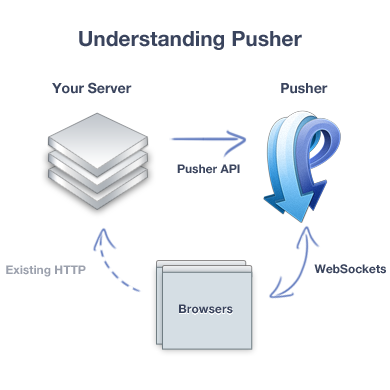
\includegraphics[scale=0.5]{image/pusher-explained.png}

Pusher creates channels that can be both listened and published to. If multiple devices are connected to the same channel, they will receive any messages sent to the channel almost simultaneously. Pusher offers a free account(an account is needed to use the system) which offers all the basic functionality we need, with up to 20 connections and 3 million messages per month

\subsubsection{PubNub}


\includegraphics[scale=0.4]{image/pubnub-logo.png}

Like Pusher, PubNub is a push service hosted in the cloud. It is written entirely in C, which gives it extremely fast performance and enables it to push over 1 million messages a second. It offers great documentation and support for the most popular libraries on both the client and server side and its in widespread use.

Like Pusher it relies on channels for communication which you can subscribe and publish to, and in essence the two solutions work in the same intuitive way. PubNub offers a free account with 1 million messages a month and up to 100 connections.

\subsubsection{Other Technologies}
We considered other similar alternatives as well, like Socket.io, Vert.x and Akka. But they either lacked support for the technologies we have chosen for the system, or lacked the extensive documentation and widespread use that Pusher and PubNub provides. We were also left with the impression that we would spend more time implementing these services than if we opted for either Pusher or PubNub.

\subsubsection{Conclusion}
Pusher and PubNub are both great systems that are widely used and they both offer extensive documentation. They cover the specific functionality we need for this project, which is to replicate the changes on both the client and server side. They both offer free accounts with more than enough connections and messages each month to cover our needs. So this decision will come down to our gut feeling. 

As none of the developers have any experience in using either system, the most important factor for this decision is that the system is well documented and easy to use. During research it became apparent that PubNub is the most widespread solution as of today. If we run into any problems implementing and using the system, it is likely someone has already provided a solution for it. So the decision ultimately fell on using PubNub.


\subsection{Google Drive}

\section{Development Methodology}
\subsection{Agile vs Waterfall}
The waterfall method focus on planning the future in detail. It follows the principle of “Big Design Up Front”. It relies on the fact that you are able to report exactly what features that are going to be implemented and tasks are planned for the entire length of the project. It forces you to specify all the requirements early in the development, when you actually know the least about the project and the problems that are to be solved. The rationale behind this is that time spent early on making sure requirements and design are correct saves you much time and effort later. A development team using the waterfall method will only consider to implement the most valuable changes, as changes in this process are time consuming and often requires that completed work is started over. The method places a lot of emphasis on documentation. 

Agile methods, as opposed to the predictive methods, are designed to plan for changes in the requirements and features of a project. It emphasises on working code as primary measure of progress, instead of extensive documentation of for example the requirements. Agile methods consists of iterative and incremental steps in the development process, where requirements and solutions evolve through the course of the project. Requirements are bound to change, either because the customer didn't understand the problem in the beginning or because they would like to add new features. Agile methods facilitates the ability to accommodate these changes. Most agile methods includes delivering a working product in incremental stages, and gives the customer something to relate to during the developments process.

The CHAOS Manifesto is a survey published by the Standish Group each year and it measures the success of IT- projects. It divides the projects into 3 groups; Success, meaning it completed on time and budget, with all features and functions as specified. Challenged, meaning it  completed, but was over cost, over time, and/or lacking all of the features and functions that were originally specified. Failed, meaning the project was abandoned or cancelled at some point and thus became a total loss.

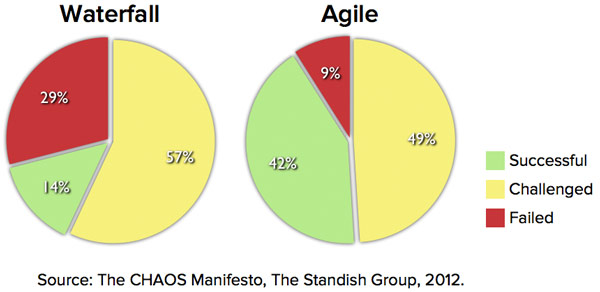
\includegraphics[scale=0.3]{image/Agile-Waterfall.jpeg}

As the figure illustrates, agile methods although not perfect by any means, more often result in products that are successful(the method used for measuring the success of a project is to some degree debated, but the results serves a purpose nevertheless).

\subsection{Agile Methods}
There exists a lot agile methods for software development, and although all of them follow the basic principles of agile development, they differ in a lot of areas. Following is a detailed description of three different agile methods.

\subsubsection{Scrum}
Scrum is an iterative, incremental software development model with several short sprints - complete small sets of tasks each sprint.

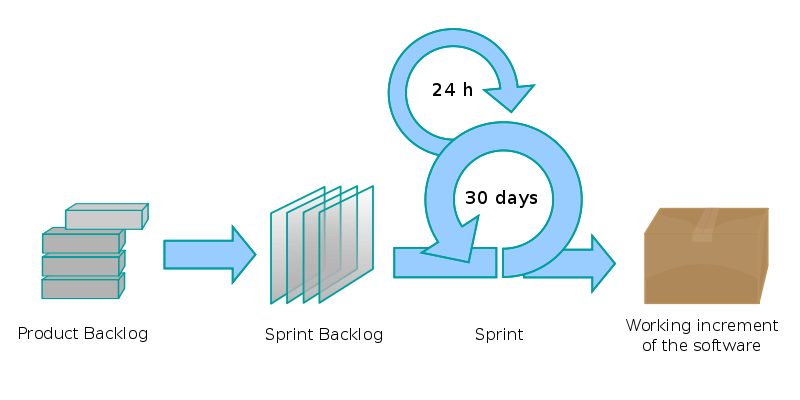
\includegraphics[scale=0.3]{image/Scrum_process.png}

The Roles: 
\begin{itemize}

\item The Scrum master, who is responsible for leading the process and to enforce the Scrum rules onto the team. He has to make sure that the development team does not overestimate what they can handle during one sprint. He leads the scrum meetings and enlightens and handles obstacles that may appear. 

\item The product owner, represents the stakeholders and is the voice of the customer.

\item The development team, is responsible for delivering potentially shippable product increments at the end of each Sprint. A development team is made up of 3–9 people with cross-functional skills.

\end{itemize}

The Sprints:
\begin{itemize}

\item Normally last from 7 to 30 days .
\item Starts with a planning meeting, where tasks are identified and goals for the sprint is set.
\item Product owner tells the team what tasks should be done in the sprint.
\item The tasks comes from a prioritized list of requirements called the backlog.
\item The team determines what is possible based on this and records this in a sprint backlog.
\item The goals should not be changed during the sprint.

\end{itemize}

The Scrum process is well suited for projects where its difficult to plan too far ahead, where at least some of the aspects of the project are unknown. Its a versatile process which is gives you the ability to handle changes in the requirements and demands from the customer. It allows for the developers to work on different parts of the project at the same time. The design, requirements of the system are not set in stone from the start, and are allowed to evolve during the process. The process delivers unfinished versions at the end of each sprint, which gives the customer a chance to try the system and give continuous feedback to the developers.

The Scrum process is somewhat complex, and it will take time to properly learn and execute the method. You also have to decide on what type of Scrum you are going to use, as there exists multiple forms of Scrum. This can prove to be a time consuming process. And even though the team members know Scrum, they will have to learn the version of scrum decided upon, if it turns out to differ from the one they are used to.
\footnote{\url{http://en.wikipedia.org/wiki/Scrum_(development)}}

\subsubsection{DSDM Atern}
DSDM(Dynamic System Development Method) is an agile software development method, and it was originally meant to provide some discipline to the Rapid Application Development method. The most recent version was launched in 2007 in an effort to make DSDM tool and technique independent, and its called Atern. 

DSDM is an iterative and incremental approach that embraces principles of agile development, including continuous user/customer involvement. It enforces you to deliver incremental versions of the product to the customer, where the main criteria of acceptance is that it meets the current business needs of the customer. It follows the principle that it is always better to deliver something “good enough” early than to deliver everything “perfect” in the end.

DSDM as a method fixes costs, quality and time at the beginning of the project. Through a prioritization method called the “MoSCoW Method”, with musts, shoulds, coulds and won’t haves, it adjusts the scope of the project to meet the given time frame. This allows the development team to focus on the critical functions of the system rather than delivering a perfect system. The method puts a strong focus on actively involving the customer in the development, and continually confirm the solution.

The principle-list of DSDM is quite long and complex. For a team that is not experienced in using the method, the process of learning the method will be time consuming. Also, always having to display the progress to the customer can be time consuming and hinder the development effort. 
Testing is central and shall be done through the whole development process.
\footnote{\url{http://en.wikipedia.org/wiki/DSDM}}

\subsubsection{Extreme Programming}
Extreme programming, hereby referred to as XP, is an agile method designed to reduce cost of changes in requirements by having multiple short development cycles. It includes elements such as pair- programming, extensive code review and unit testing of all the elements of the code. It emphasises frequent communication with the customer and between the developers.

The method embraces changes in the requirements of the project, and it doesn't attempt to define a stable set of requirements at the beginning of the project. In XP a representative for the customer is always available on site to answer any questions the developers might have. It also focuses on frequent releases of working code which serves as checkpoints where the customer can add new requirements.
 
XP puts a lot of focus on the code of the project, the advocates of XP argues that the code is the only truly important product of the system development process. XP as a process does not produce a lot of written documents during the development of the project. In XP programmers are expected to assume a unified client viewpoint and focus on coding rather than documentation of compromise objectives and constraints.
\footnote{\url{http://en.wikipedia.org/wiki/Extreme_Programming}}

\subsection{Conclusion}
If all of the requirements of this project were known in advance and provided by the customer, or the features of the finished product was known and unlikely to change, the waterfall method might be the way to go. But this is a prototype, proof of concept type of project where very little is known about the final product. We were certainly not presented with a finished set of requirements at the beginning of the project, and the requirements we settle on before we start the implementation are also more than likely to change during development. These kind of changes in a waterfall process will be time consuming. Thats why we think that an agile development method will be the best choice for this project.

All of the agile methods described above exhibits properties that will come in useful in this project. They are all based on iterative and incremental development steps, delivering prototypes for the customer to test after each step. This will give the customer a chance to try out unfinished versions of the product and give continuous feedback throughout the project. It can also help the customer to identify new features that they would like to add. They also allows the customer to decide which features to implement in each step, ensuring that the final product will contain the features the customer really need.

The agile methods embrace changes in the requirement and provides ways to handle those changes. They also encourage tight and continuous communication with the customer, which is important to be able to deliver a product that the customer is satisfied with

Of the three methods the group members are most familiar with the Scrum process. The DSDM method is complex and will take a considerable effort to learn and execute correctly. As none of the group members have used DSDM, and we have a limited amount of time in this project, DSDM is of the table. 

XP puts a lot of focus on the code, and delivers a minimal set of documents. We are to write an extensive report about the project, and document every part of it, including compromises and assumptions made. The amount of code in this project will be limited and none of the team members have any experience in working with XP. As a result, XP seems like a bad fit for our project.

The Scrum process does not put as much focus on documentation as the waterfall process, but we think that the amount of documentation produced during the Scrum process will be satisfactory for the report. It will take time to learn how to execute Scrum properly, but since all of the group members are familiar with the basics of process, we think it won’t be too time consuming and worth the effort. The final decision then is to use Scrum as a development method for this project.

\section{Software Testing}

\subsection{Testing Methods}
The purpose of software testing is to uncover software bugs in the system and to document that the system meet the requirements and functionality that was agreed upon for the system. Testing can be implemented at any stage in the development process, traditionally it is performed after the requirements have been defined and the implementation is completed. In agile development processes however, the testing is an ongoing process. The chosen development methodology will in most cases govern the type of testing implemented in a given project.

Software testing methods are traditionally divided into white- and black- box testing. They differ mainly in how the test engineer derives test cases.

\subsubsection{White- Box Testing}
White- box testing focus on the internal structures of a system. It uses this internal perspective to derive test cases. White- box testing is usually done at unit level, testing specific parts or components of the code. 

\subsubsection{Black- Box Testing}
Black- box testing handles the software as a black- box, meaning it observes the functionality the system exhibits and not the specifics on how it is implemented. The tester only needs to be aware of what the program is supposed to do, he doesn't need to know the specifics on how the functionality is implemented in the code. Black- box testing checks to see if the functionality of the program is according to the agreed upon requirements, both functional and nonfunctional. 

\subsubsection{Test Driven Development}
The principle behind TDD is to develop the code incrementally, along with test for that increment. You don’t move on until the code passes its test. The tests are to be written before you actually implement the new functionality. The process helps programmers clarify their ideas of what a code segment is actually supposed to do. The process is often used in agile development methods.
Benefits from TDD include: 
\begin{itemize}

\item Code coverage, every code segment should be covered at least one test.

\item Regression testing, check to see if changes in the code have not introduced new bugs.

\item Simplified debugging, when a test fails it should be obvious where the problem lies, no need for a debug tool.

\item System documentation, the tests themselves act as a form of documentation that describe what the code should be doing.

\end{itemize}

\subsubsection{Automated Tests}
Automated offers the ability to automatically do regression tests, i.e. testing to uncover if any new code has broken a test that previously passed. If we opt for manual testing regression testing will be very time consuming as every test done so far has to be done over again. With an automated testing framework this job will be a lot easier as you can run a great number of tests in a matter of seconds. Most development languages offers libraries for automated testing.


\subsection{Testing Levels}
Testing can be done at many different levels and in different stages in the development process. Following is the most common partitioning of testing levels and a description on each of them.

\subsubsection{Unit Testing}
Unit testing aims to check specific components, such as methods and objects. Typically you will be testing objects, and you should provide test coverage of all the features of that object. Its important to choose effective unit test cases, that reflect normal operation and they should show that the specific component works. Abnormal inputs should also be included to check if these are processed correctly.

\subsubsection{Component Testing}
Tests bigger components of the system, and their interfaces(communication with other components). Made up of several interacting objects. Component testing is mainly a tool to check if component interfaces behaves according to its specification.

\subsubsection{System Testing}
In a given development project there may be several reusable components that have been developed separately and COTS systems, that has to be integrated with newly developed components. The complete system composing of the different parts is tested at this level. Components developed by different team members or groups may also be integrated and tested at this stage.

\subsubsection{Release Testing}
Release testing is the process of testing a particular release of the system that is intended for use outside of the development team. Often a separate team that has not been involved in the development perform this testing. These kind of tests should focus on finding bugs in the complete system. The objective is to prove to the customer that the product is good enough. This kind of testing could either be based on the requirements of the system or on user scenarios.

\subsubsection{User Testing}
This is a stage in the testing process in which users or customers provide feedback and advice. This could be an informal process where end- users experiment with a new system too see if they like it and that it conforms to their specific needs. Testing on end- users is essential for achieving success in a software process as replicating the exact working environment the system will be used in is difficult to achieve during development. The end users can help provide feedback on how specific functionality will work in an actual work environment.

Another form of user testing involves the customer and its called acceptance testing. Its a process where the customer formally tests a system to decide whether or not it should be accepted, where acceptance implies that payment for the system should be made. Acceptance testing is performed after the release testing phase.


\section{Code conventions}
\section{Similar solutions}
\chapter{Project management}

\section{Project name}
Project name is important project identificator. It should summarize main project goal or functionality. In real project, is often a trademark, or reflects the name of the company.

In this section, we will describe the process of choosing a name for the project. First of all, we made a list of words, that we can use in the project name. These words describe project funcionality or goal.

Words that can be used in project name: master, console, web, text, keyboard

We used the list of words and brainstorming session on a meeting for compiling a list of project name candidates:

Candidate project names: console 2.0, wonsole, wensole, websole, werminal, interCLI

After discussion we chose the name \emph{Wonsole}. Project name can be sometimes little confusing, so we added the subtitle: \emph{The new web console for power users.}

\section{Team roles}
\begin{tabularx}{\textwidth}{ | l | X | l | }
  \hline
  \textbf{Role} & \textbf{Description} & \textbf{Assignee} \\ 
  \hline
  Team leader & Is responsible for administrative tasks and makes the final decisions. & Ivo \\ 
  \hline
  Scrum Master & Shields the development team from external distractions and enforces the Scrum scheme.  & Ivo \\ 
  \hline
  Customer Contact & Handles communication with the customer. The customer should contact this person regarding general requests, questions and reminders. & Ivo (backup Martin) \\ 
  \hline
  Advisor Contact & Handles communication with the advisor. The advisor should contact this person regarding general requests, questions and reminders.  & Ivo (backup Martin) \\ 
  \hline
  System Architect & Is responsible for the system architecture including distinctions and relations between subsystems and general code design choices. & Martin \\ 
  \hline
  Code Master & Overall responsible for code management and structure. Managing branches in Git repository. & Oddvar  \\ 
  \hline
  GUI Designer & Is responsible for the layout and design of graphical user interfaces. & Oddvar \\ 
  \hline
  Test Manager & Is responsible for testing including unit tests, integration tests and usability tests. & Oystein \\ 
  \hline
  Report Manager & Is responsible for delegating and overseeing work on the project report. & Martin \\ 
  \hline
  Customer Representative & Participates in regular meetings to discuss the progress, project status and future tasks. Represents the customer. & Peder Kongelf \\ 
  \hline
  Customer Technical Advisor & May be consulted about technical aspects of the project. & Stig Lau \\ 
  \hline
  Advisor & Serves as a one-man steering committee for the project. & Meng Zhu \\ 
  \hline
  Meeting Secretary & Is responsible for making sure notes get written and sent after each meeting with the advisor and customer. & Oddvar \\ 
  \hline
  Quality Assurance Manager &  & Oystein \\ 
  \hline
  Weekly Report Writer & Is responsible for finalizing the weekly report(s) for the advisor and customer, and getting these delivered for approval. Also responsible for meeting agendas and their delivery. & Oystein \\ 
  \hline
  Time Keeper & Responsible for making sure that everybody is logging their work, and logging team activities. & Oddvar \\ 
  \hline
\end{tabularx}

\section{Quality Assurance}
\subsection{Communication rules}
To prevent misunderstanding in communication and

\begin{tabularx}{\textwidth}{ | c | X | }
  \hline
  meeting & scheduled at least 48 hours before, confirmation within 24 hours before meeting required \\ \hline
  documents for the meeting & 24 hours before \\ \hline
  email communication & contact person directly, google groups is just internal \\ \hline
  response from the team & within 8 hours \\ \hline
  response from customer & within 24 hours \\ \hline
\end{tabularx}

\section{Risks}
\begin{tabularx}{\textwidth}{ | l | X | l | l | }
  \hline
  \textbf{\#} & \textbf{Risk} & \textbf{Probability} & \textbf{Impact} \\ \hline
  1 & Not getting a fifth party member & M & Significant \\ \hline
  2 & Obtrusive health/family/personal issues for team members & L & Significant \\ \hline
  3 & Low morale in team & M & Significant \\ \hline
  4 & Interfering workload from other activities & H & Minor \\ \hline
  5 & Miscommunication with customer & M & Critical \\ \hline
  6 & Changes in customer requirements & M & Significant \\ \hline
  7 & Errors in project plan & M & Significant \\ \hline
  8 & Failure of communication in team & M & Critical \\ \hline
  9 & Failure of time management & H & Critical \\ \hline
 10 & Errors in workload estimation and distribution & H & Critical \\ \hline
 11 & Failure of online storage systems and services & L & Significant \\ \hline
 12 & Failure of personal computers & M & Significant \\ \hline
 13 & Infeasibility of project as a whole & L & Critical \\ \hline
 14 & Inability to find potential users and test subjects & M & Significant \\ \hline
\end{tabularx}


\begin{tabularx}{\textwidth}{ | l | X | }
\hline
\textbf{Risk \#} & 1 \\ \hline
\textbf{Activity} & All \\ \hline
\textbf{Risk Factor} & Not getting a fifth party member \\ \hline
\textbf{Impact} & Significant \\ \hline
\textbf{Consequence} & Increased workload for all remaining party members on all activities \\ \hline
\textbf{Probability} & Medium \\ \hline
\textbf{Countermeasures} & \begin{itemize}
  \item  Contact advisor about the dropped party member, try to get assigned a new member.
  \item Take the missing person into account in planning phase.
\end{itemize}  \\ \hline
\textbf{Deadline} & Intro/Planning (Ultimately in the hands of course staff) \\ \hline
\textbf{Responsible} & Project leader \\ \hline
\end{tabularx}



\begin{tabularx}{\textwidth}{ | l | X | }
\hline
\textbf{Risk \#} & 2 \\ \hline
\textbf{Activity} & All \\ \hline
\textbf{Risk Factor} & Obtrusive health/family/personal issues for team members \\ \hline
\textbf{Impact} & Significant \\ \hline
\textbf{Consequence} & Increased workload for all remaining party members on all activities \\ \hline
\textbf{Probability} & Low  \\ \hline
\textbf{Countermeasures} & \begin{itemize}
  \item Implement buffers in project plan.
  \item Team members should make their work resumable by another member.
\end{itemize}  \\ \hline
\textbf{Deadline} &  None \\ \hline
\textbf{Responsible} & Project leader \\ \hline
\end{tabularx}

\begin{tabularx}{\textwidth}{ | l | X | }
\hline
\textbf{Risk \#} & 3 \\ \hline
\textbf{Activity} & All \\ \hline
\textbf{Risk Factor} & Low morale in team \\ \hline
\textbf{Impact} & Significant \\ \hline
\textbf{Consequence} & Decreased overall project quality \\ \hline
\textbf{Probability} & Medium  \\ \hline
\textbf{Countermeasures} & \begin{itemize}
  \item Frequent contact between team members
  \item Avoid team members overworking
  \item Focus on general team dynamics advice from advisor
\end{itemize}  \\ \hline
\textbf{Deadline} &  None \\ \hline
\textbf{Responsible} & Project leader \\ \hline
\end{tabularx}





\begin{tabularx}{\textwidth}{ | l | X | }
\hline
\textbf{Risk \#} & 4 \\ \hline
\textbf{Activity} & All \\ \hline
\textbf{Risk Factor} & Interfering workload from other activities \\ \hline
\textbf{Impact} & Low \\ \hline
\textbf{Consequence} & Work on the project is shifted in time, space and responsibility \\ \hline
\textbf{Probability} & Very High \\ \hline
\textbf{Countermeasures} & \begin{itemize}
  \item Plan ahead with respect to existing schedules
  \item Inform the group of other activities
\end{itemize}  \\ \hline
\textbf{Deadline} &  None \\ \hline
\textbf{Responsible} & Project leader \\ \hline
\end{tabularx}


\begin{tabularx}{\textwidth}{ | l | X | }
\hline
\textbf{Risk \#} & 5 \\ \hline
\textbf{Activity} & All \\ \hline
\textbf{Risk Factor} & Miscommunication with customer \\ \hline
\textbf{Impact} & Critical \\ \hline

\textbf{Consequence} & -The project is not developed as the customer wants it
-Work has to be done over \\ \hline
\textbf{Probability} & Very High \\ \hline
\textbf{Countermeasures} & \begin{itemize}
  \item Weekly customer meetings
  \item Share as much information as possible with customer at all stages
\end{itemize}  \\ \hline
\textbf{Deadline} &  None \\ \hline
\textbf{Responsible} & Customer Contact \\ \hline
\end{tabularx}

\begin{tabularx}{\textwidth}{ | l | X | }
\hline
\textbf{Risk \#} & 6 \\ \hline
\textbf{Activity} & Planning, Requirements, Implementation \\ \hline
\textbf{Risk Factor} & Changes in customer requirements \\ \hline
\textbf{Impact} & Significant \\ \hline
\textbf{Consequence} & Work has to be done over  \\ \hline
\textbf{Probability} & Medium \\ \hline
\textbf{Countermeasures} & \begin{itemize}
  \item Design the prototype with possible modifications in mind.
  \item Try to get information on possible changes from the customer.
\end{itemize}  \\ \hline
\textbf{Deadline} &  None \\ \hline
\textbf{Responsible} & Customer Contact \\ \hline
\end{tabularx}


\begin{tabularx}{\textwidth}{ | l | X | }
\hline
\textbf{Risk \#} & 7 \\ \hline
\textbf{Activity} & Implementation \\ \hline
\textbf{Risk Factor} & Errors in project plan \\ \hline
\textbf{Impact} & Significant \\ \hline
\textbf{Consequence} & Work on the plan and implementation have to be redone  \\ \hline
\textbf{Probability} & Medium \\ \hline
\textbf{Countermeasures} & \begin{itemize}
  \item Review the project plan frequently for consistency
  \item Share plan with customer
\end{itemize}  \\ \hline
\textbf{Deadline} &  Planning \\ \hline
\textbf{Responsible} & Project Leader \\ \hline
\end{tabularx}

\begin{tabularx}{\textwidth}{ | l | X | }
\hline
\textbf{Risk \#} & 8 \\ \hline
\textbf{Activity} & All \\ \hline
\textbf{Risk Factor} & Failure of communication in team \\ \hline
\textbf{Impact} & Critical \\ \hline
\textbf{Consequence} & Failure of unification of the work, uneven workloads, decreased project quality  \\ \hline
\textbf{Probability} & Medium \\ \hline
\textbf{Countermeasures} & \begin{itemize}
  \item Frequent internal meetings
  \item Sharing of work internally
\end{itemize}  \\ \hline
\textbf{Deadline} &  None \\ \hline
\textbf{Responsible} & Project Leader \\ \hline
\end{tabularx}

\begin{tabularx}{\textwidth}{ | l | X | }
\hline
\textbf{Risk \#} & 9 \\ \hline
\textbf{Activity} & All \\ \hline
\textbf{Risk Factor} & Failure of time management \\ \hline
\textbf{Impact} & Critical \\ \hline
\textbf{Consequence} & Parts of project are rushed or not finished in time \\ \hline
\textbf{Probability} & High \\ \hline
\textbf{Countermeasures} & \begin{itemize}
  \item Put in as much work as possible as early as possible
  \item Implement buffers in project plan
\end{itemize}  \\ \hline
\textbf{Deadline} &  None \\ \hline
\textbf{Responsible} & Project Leader \\ \hline
\end{tabularx}

\begin{tabularx}{\textwidth}{ | l | X | }
\hline
\textbf{Risk \#} & 10 \\ \hline
\textbf{Activity} & All \\ \hline
\textbf{Risk Factor} & Errors in workload estimation and distribution \\ \hline
\textbf{Impact} & Critical \\ \hline
\textbf{Consequence} & Uneven workloads, rushed or unfinished parts of project \\ \hline
\textbf{Probability} & High \\ \hline
\textbf{Countermeasures} & \begin{itemize}
  \item Implement buffers in project plan
  \item Avoid relying too much on rigid plans
  \item Allow for redistribution of work when necessary
\end{itemize}  \\ \hline
\textbf{Deadline} &  Planning \\ \hline
\textbf{Responsible} & Project Leader \\ \hline
\end{tabularx}




\section{Meetings}
\section{Lectures}
\section{Issues}


\section{Project plan}
\subsection{Sponsor/customer}
\subsection{Background}
\subsection{Gantt diagram}
\section{Team structure}
\subsection{Roles}
 
\section{Risks}
\section{Architecture}
\section{Scrum}
\section{Quality Assurance}

\section{Domain choosing}
Domain ideas:
project management tool (ehm. redmine)
warehouse
airport / travel agency
cash registers (not interesting)
bank
school information system (boring)
time management system (aka calendar)
facebook console (unreal)
mail interface (gmail is too good, not useful)
photo gallery (limited)
music library (limited)
physician system (treatments, prescriptions, add person)
tax form (boring)
Building management (boring)
Library

(ehm. redmine) 
warehouse 1
1
bank 3 3
(aka calendar) 2
(treatments, prescriptions, add person) 1
Library 2 2 3

Ivo	Martin	Oddvar	Oystein	Total
project management tool	3		2		5
warehouse			1		1
airport / travel agency		1			1
bank		3		3	6
time management system	2				2
physician system	1			1	2
Library		2	3	2	7




Top3:
library
authors, books(location, state), book management, employees, user management, order new books, 

bank
accounts, transfer money, deposits, loans, customer management, employees

project management
projects, issues, work done on issues, workers, sprints, reports, 

interesting	simple to understand	complex enough	ease workflow	existence of power user	total
library	2	3	1	2	Y	8
bank	2	3	2	2	Y	9
project management	1	2	3	2	Y	8



project management
+ usefulness
+ field of study
- boring

library
+ libraries in campus, employees
- simple

bank
- unknown ground


library	project management	bank
martin	3	2	1
oddvar	3	2	1
ivo	2	3	1
oystein	3	1	2
total	11	8	5



Criteria:
Interesting and simple enough for test subjects to understand. something they meet in everyday life
Complicated enough to demonstrate the problem.
Console has to be useful in the domain, ease the workflow
Object oriented design
Existence of power user, that will use the console

Customer ideas:
car models
finn.no
health sector
human resources (people, how they are related, symptoms, how much money and what they own - advanced domain graph). 
contact lists (peder)


write these things to the report


Future:
batch operations
undo the commands
save command for object attribute editing
what about object operations?
transaction support


\chapter{Requirements}
\section{Usecases/user stories}
\subsection{Planning}
\section{Sequence Diagrams}
\section{Prioritization}
\section{Functional Requirements}
\section{Nonfunctional Requirements}


\section{Test Plan}
This chapter will introduce the overall test plan for this project, and it is based on the IEEE 829 Standard for Software Test Documentation[link to reference]. Some parts of the standard was not deemed to be appropriate for this project and not included as a result. The purpose of this document is to structure the way tests are performed and recorded, assign responsibilities for the testing process as a whole, and to give an outline for the schedule of when the different tests should be performed.

\subsection{Testing Approach}
The testing methods used for this project is discussed in detail in the pre- study. To sum up, we have opted to utilize both black and white box testing in this project. We will write and run unit tests throughout the implementation process together with an automated test framework. The test cases included in the report will be component, system, user and acceptance tests. If additional requirements are added to the system during the Scrum process, new test cases will be created to test the desired functionality.

\subsubsection{Non- Functional Requirements}
The aren’t many non- functional requirements that are essential in this project. It is a proof of concept type of project and the main goal is to prove that the solutions we come up with will get the job done. As a result, tests for common non- functional requirements like performance and security will not be included in the test cases. 

One non- functional requirement worth writing tests for though is usability. The object of the project is to deliver a system that eases the workflow of specific users, and to achieve this we need to develop a system with a large degree of usability. Thats why usability tests will be included in the test cases, in the form of user testing(interviews).

\subsubsection{Testing Process Timeline}
Figure~\ref{figure:testOutline} outlines when the different tests will be performed during the Scrum process. Unit testing will be done throughout the development process in every sprint. Every part of the code implemented should have its own unit tests. Component testing will be done as separate components are finished, typically towards the end of the sprints. Acceptance testing with the customer will be performed in the sprint demo at the end of each sprint. At these demos it will be tested whether the agreed upon functionality for that sprint is actually implemented. System testing will be performed when we have an entire system to test, i.e. when we have implemented some parts of each component needed for the entire system to work. This will likely not be the case until the end of the second sprint. User testing will also be performed in the later sprints, when we have a complete system to present to the test users. Release testing will be performed at the end of the last sprint, to see if the agreed upon functionality for the entire project is indeed present in the system.

\begin{figure}
\centering
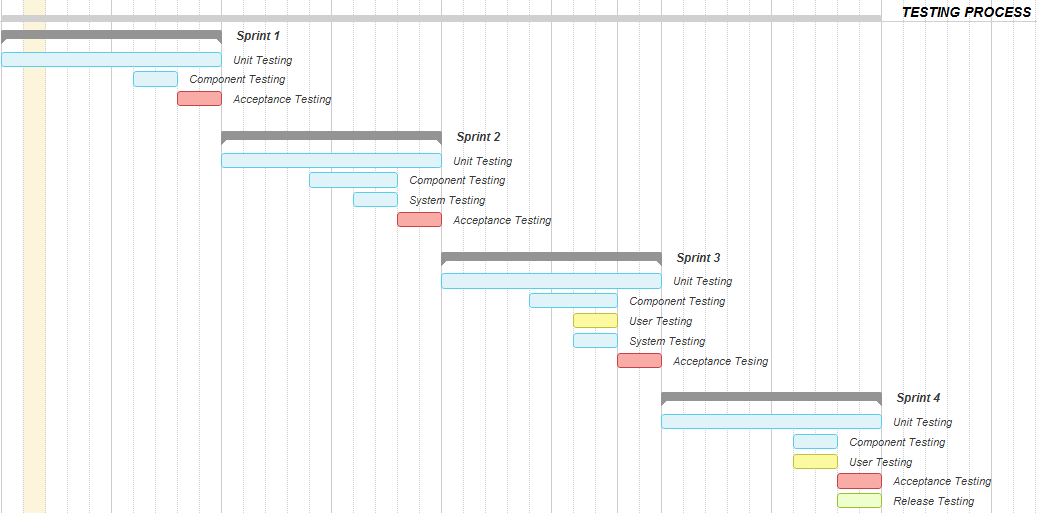
\includegraphics[width=6in]{image/testingProcess.png}
\caption{Testing Process Timeline}
\label{figure:testOutline}
\end{figure}

\subsection{Templates}
The templates stated in Table~\ref{table:testcase} and Table~\ref{table:testreport} will be used to create test cases and to record the results of them.

\begin{table}
\caption{Test Case Template}
\centering
\begin{tabular}{ l l }
\hline
 Item            & Description                                                              \\ 
\hline
 Description     & Description of requirement                                               \\ 
 Tester          & The person responsible for performing the specific test                  \\ 
 Preconditions   & The condition that has to be fulfilled before the execution of this test \\ 
 Feature         & The feature of the system that is to be tested                           \\ 
 Execution steps & Steps to be executed in this test case                                   \\ 
 Expected result & The expected result of the test                                          \\
\hline
\end{tabular}
\label{table:testcase}
\end{table}

\begin{table}
\caption{Test Report Template}
\centering
\begin{tabular}{ l l }
\hline
Item        & Description                             \\ 
\hline
Test ID     & The ID of the given test                \\ 
Description & Description of the requirement          \\ 
Tester      & The person executing the test           \\ 
Date        & The date the test was performed         \\ 
Result      & The result of the test, success or fail. Comment will be added if deemed needed \\
\hline
\end{tabular}
\label{table:testreport}
\end{table}

\subsection{Responsibilities}
The test manager is the one with overall responsibility of the quality of the test plan, and that it will be executed according to the schedule. The person writing test cases and recording test results is responsible for adhering to the templates included in this document.

Each person is responsible for creating unit tests for their own code, and to run these with the automated test framework during development. This will be done to perform continuous testing of the system, and uncover if any new code break some of the previous tests.

We will mainly use someone different to perform the actual test cases than the person who wrote the specific code segment. This is done to achieve as little ownership of the code as possible on part of the tester. But as we are short on manpower and time we can’t guarantee that this is always the case. 

The test cases will be performed towards the end of each sprint when the relevant functionality is implemented. The test will be performed at a time which allows the developers to fix any uncovered bugs in the system before the sprint is ended. 

\subsection{Test Criteria}
A test is considered passed when it achieves the expected result. A test will be considered to have failed if the result of the test differs from the expected one. If we feel a pass/fail of a specific test needs an explanation this will be noted as a comment in the result.
\chapter{Overall System Design}
\section{Database}
\section{GUI}


\chapter{Sprints}
\section{Design}
\section{Planning}
\section{Duration}
\section{Goals}
\section{Testing}


\chapter{Conclusion}



\end{document}